\documentclass[11pt,a4paper]{article}
\usepackage[margin=2.5cm]{geometry}
\usepackage{graphicx}
\usepackage{subcaption}

\graphicspath{{figures/}}

\title{Measurement and Analysis of Pulse-oxi and ECG Signals\\
       \large Intermediate report}
\author{Kirill Rybkov, Malek Galal Hamed Mohamed Ghanem}
\date{2nd October 2026}

\begin{document}
\maketitle

% =====================================================================
\section{Raw data}
% =====================================================================
% Manual 2.2.1a Present the measured four signals in four sub-figures. Limit the presented
% range to 10 seconds.
\paragraph{(a)} Figure~\ref{fig:raw} shows the four raw signals ($f_s = 1024$~Hz) over
$t = 35$--45~s, a stretch without movement distortion in the ECG. The pulse-oxi signal sig-P
(pleth) comes from the finger clip, and the ECG signals sig-R, sig-L and sig-F were measured on the
right wrist, left wrist and left ankle, relative to the right ankle.

\begin{figure}[!htb]
  \centering
  \begin{subfigure}{0.49\textwidth}\centering
    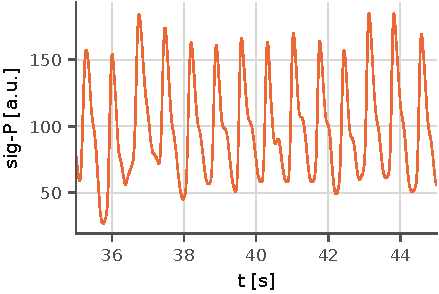
\includegraphics[width=\linewidth]{raw_P}\caption{sig-P}\label{fig:raw-P}
  \end{subfigure}\hfill
  \begin{subfigure}{0.49\textwidth}\centering
    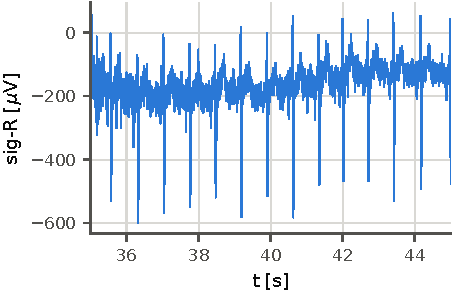
\includegraphics[width=\linewidth]{raw_R}\caption{sig-R}\label{fig:raw-R}
  \end{subfigure}\\[4pt]
  \begin{subfigure}{0.49\textwidth}\centering
    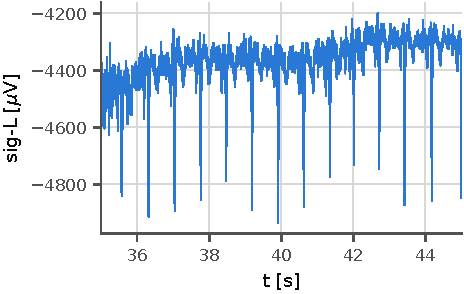
\includegraphics[width=\linewidth]{raw_L}\caption{sig-L}\label{fig:raw-L}
  \end{subfigure}\hfill
  \begin{subfigure}{0.49\textwidth}\centering
    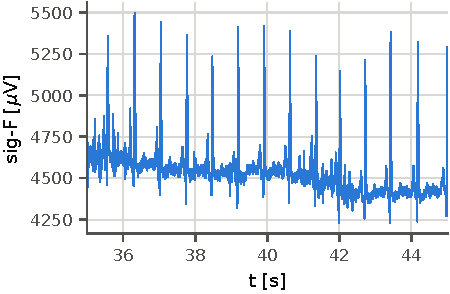
\includegraphics[width=\linewidth]{raw_F}\caption{sig-F}\label{fig:raw-F}
  \end{subfigure}
  \caption{Raw signals, $t = 35$--45~s ($f_s = 1024$~Hz). sig-P in arbitrary units (a.u.), the
  ECG signals in $\mu$V.}
  \label{fig:raw}
\end{figure}

% Manual 2.2.1b Comment on the prominent features you observe in 2-3 sentences.
\paragraph{(b)} All four signals repeat with the heartbeat (about 84~bpm). The ECG
channels show a sharp spike every beat (negative in sig-R and sig-L, positive in sig-F) on top
of DC offsets (about $\pm 4500$~$\mu$V in sig-L and sig-F), slow baseline drift and high-frequency noise. sig-P is a
smooth wave whose peaks lag the ECG spikes by about 0.4~s.

% =====================================================================
\section{Fourier transform of the raw data}
% =====================================================================
% Manual 2.2.2a Perform a Fourier transform on the four signals. Present the amplitude of the
% frequency spectrum in four sub-figures. Limit the frequency axis to 0-80 Hz range.
\paragraph{(a)} Figure~\ref{fig:fft} shows the amplitude $2|X[k]|/N$ of the DFT
\[
  X[k] = \sum_{n=0}^{N-1} x[n]\,e^{-j2\pi kn/N},
\]
calculated with the FFT over the same 10~s window as Figure~\ref{fig:raw} ($N = 10240$,
$\Delta f = f_s/N = 0.1$~Hz) after removing the mean (DC offset).

\begin{figure}[!htb]
  \centering
  \begin{subfigure}{0.49\textwidth}\centering
    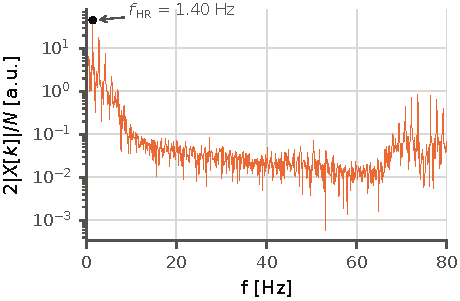
\includegraphics[width=\linewidth]{fft_P}\caption{sig-P}\label{fig:fft-P}
  \end{subfigure}\hfill
  \begin{subfigure}{0.49\textwidth}\centering
    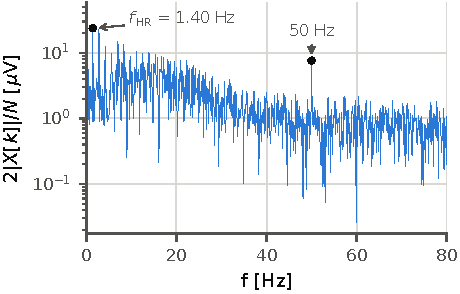
\includegraphics[width=\linewidth]{fft_R}\caption{sig-R}\label{fig:fft-R}
  \end{subfigure}\\[4pt]
  \begin{subfigure}{0.49\textwidth}\centering
    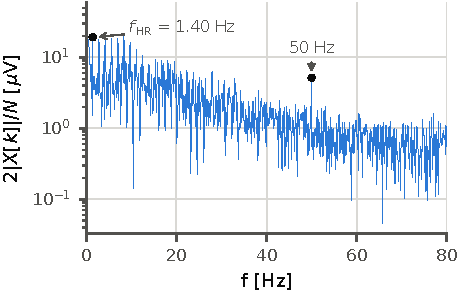
\includegraphics[width=\linewidth]{fft_L}\caption{sig-L}\label{fig:fft-L}
  \end{subfigure}\hfill
  \begin{subfigure}{0.49\textwidth}\centering
    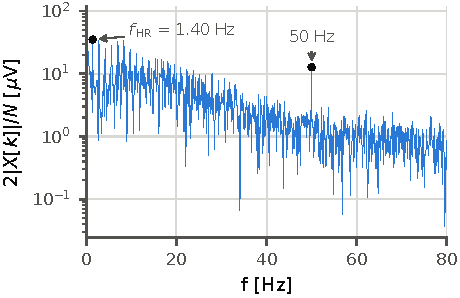
\includegraphics[width=\linewidth]{fft_F}\caption{sig-F}\label{fig:fft-F}
  \end{subfigure}
  \caption{Amplitude spectra of the raw signals, $t = 35$--45~s, 0--80~Hz (logarithmic
  amplitude axis).}
  \label{fig:fft}
\end{figure}

% Manual 2.2.2b Comment on the prominent peaks in your spectra in 2-3 sentences.
\paragraph{(b)} All spectra show a peak at $f_\mathrm{HR} = 1.40$~Hz (84~bpm) and at its
harmonics, since the heartbeat is periodic but not sinusoidal. The ECG spectra also show their
largest amplitude below 0.3~Hz, from the slow baseline drift, probably caused by breathing and changing electrode
contact, and a narrow 50~Hz line (5--13~$\mu$V) picked up from the mains.
The sig-P spectrum also shows peaks at 73.6 and 76.4~Hz ($75 \pm 1.4$~Hz), because the
oximeter output changes in steps only about 75 times per second, which
adds copies of the heartbeat lines around 75~Hz.

% Manual 2.2.2c Comment on the comparison of four spectra.
\paragraph{(c)} All four spectra share the peak at 1.40~Hz and its harmonics. The
sig-P spectrum is much narrower than the ECG spectra. Its harmonics drop from 45 to
1.1 arbitrary units (a.u.) by 7~Hz, while the ECG spectra decay slowly, up to about 30~Hz, because the sharp ECG
spikes contain more high frequencies than the smooth pulse wave. Drift and 50~Hz are clear only in
the ECG spectra, and only sig-P has the 75~Hz lines. The three ECG spectra have the same shape
and differ mainly in level, sig-F being the largest (35~$\mu$V at 1.40~Hz, against 24 and
19~$\mu$V for sig-R and sig-L).

% =====================================================================
\section{Auto-correlation}\label{sec:acf}
% =====================================================================
% Manual 2.2.3a Calculate the auto-correlations of four signals. You are advised to limit your
% auto-correlation calculations to a 5 seconds long sub-part of the signal that is around 0
% and showing least drift. Plot the results in four sub-figures. Comment on your observations
% for each sub-figure.
\paragraph{(a)} Figure~\ref{fig:acf} shows the normalised auto-correlation
$R_{xx}[n]/R_{xx}[0]$, with
\[
  R_{xy}[n] = \sum_m x[m]\,y[m-n],
\]
over $t = 36.5$--41.5~s, a 5~s window with little baseline drift, after subtracting the mean.
All four are symmetric, equal 1 at zero lag and have side peaks at multiples
of 0.72~s, the heartbeat period. The side peaks decrease with lag because fewer samples overlap.
\begin{itemize}
  \item sig-P: broad peaks with deep minima ($-0.52$) halfway between them, first side peak
        (0.80).
  \item sig-R: narrow peaks with only small dips (about $-0.1$) between them, lowest first
        side peak (0.62).
  \item sig-L: narrow peaks with the deepest dips, to $-0.2$ at $\pm 0.07$~s, first side peak
        (0.66).
  \item sig-F: narrow peaks with dips of $-0.14$, highest first side peak of the ECG channels
        (0.69).
\end{itemize}

\begin{figure}[!htb]
  \centering
  \begin{subfigure}{0.49\textwidth}\centering
    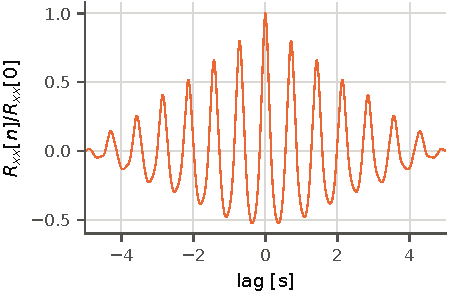
\includegraphics[width=\linewidth]{acf_P}\caption{sig-P}\label{fig:acf-P}
  \end{subfigure}\hfill
  \begin{subfigure}{0.49\textwidth}\centering
    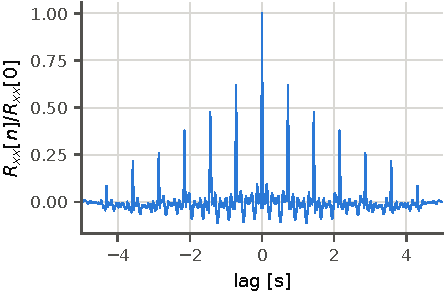
\includegraphics[width=\linewidth]{acf_R}\caption{sig-R}\label{fig:acf-R}
  \end{subfigure}\\[4pt]
  \begin{subfigure}{0.49\textwidth}\centering
    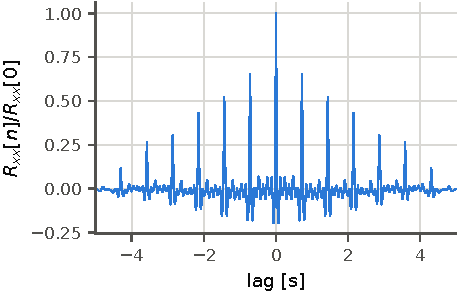
\includegraphics[width=\linewidth]{acf_L}\caption{sig-L}\label{fig:acf-L}
  \end{subfigure}\hfill
  \begin{subfigure}{0.49\textwidth}\centering
    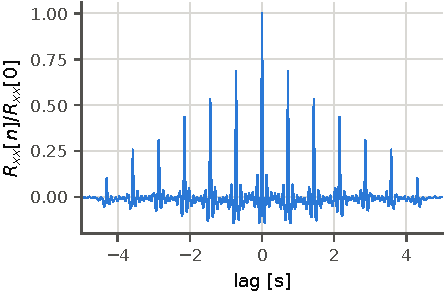
\includegraphics[width=\linewidth]{acf_F}\caption{sig-F}\label{fig:acf-F}
  \end{subfigure}
  \caption{Normalised auto-correlations, $t = 36.5$--41.5~s.}
  \label{fig:acf}
\end{figure}

% Manual 2.2.3b Compare the signals and comment on your observations.
\paragraph{(b)} All four signals have the same period, as they come from the same
heartbeat. The peaks are broad for sig-P and narrow for the ECG, like the waveforms themselves. The first
side peak is higher for sig-P (0.80) than for the ECG channels (0.62--0.69), because the
heartbeat period varies by about 20~ms, which smears the narrow ECG peaks but hardly affects
the broad sig-P peaks. The ECG channels record the same beats, so the differences in side-peak height come from
noise. Noise is different every beat and lowers the side peaks, so sig-F has the least noise
relative to its signal, then sig-L, then sig-R.

% =====================================================================
\section{Cross-correlation}
% =====================================================================
% Manual 2.2.4a Calculate the cross-correlation between sig-P and the cleanest signal out of
% the three ECG recordings. You can again limit your correlation calculations to a 5 seconds
% long sub-part of the signal that is around 0 and showing least drift. Plot the result in a
% figure. Comment on your observations in 2-3 sentences.
\paragraph{(a)} The cleanest ECG signal is sig-F, as its first auto-correlation side peak
(0.69) is higher than those of sig-R (0.62) and sig-L (0.66) (Section~\ref{sec:acf}). Its
normalised cross-correlation with sig-P, $R_{PF}[n]/\sqrt{R_{PP}[0]\,R_{FF}[0]}$ over the same
window (Figure~\ref{fig:xcorr}), repeats every 0.72~s, with maxima of 0.19 at $+0.41$~s and
0.22 at $-0.25$~s. A positive lag means sig-P is delayed, and the
$-0.25$~s maximum is the pulse of the previous beat, so the pulse peak follows the ECG spike by about
0.4~s.

\begin{figure}[!htb]
  \centering
  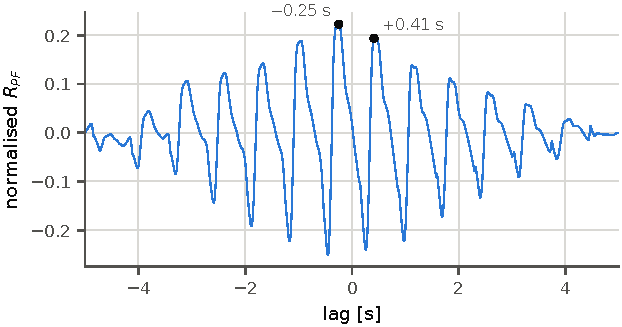
\includegraphics[width=0.65\textwidth]{xcorr_PF}
  \caption{Normalised cross-correlation between sig-P and sig-F, $t = 36.5$--41.5~s.}
  \label{fig:xcorr}
\end{figure}

% Manual 2.2.4b Compare your cross-correlation observations to your auto-correlation
% observations.
\paragraph{(b)} The cross-correlation has the same period as the auto-correlations, but
it is not symmetric and its maximum is not at zero lag. It is also much lower (0.22) than the 1 at
zero lag and the first side peaks of 0.62--0.80, because the two waveforms have very
different shapes. Its broad peaks resemble the sig-P auto-correlation instead of the narrow
ECG peaks.

% Manual 2.2.4c Conclude with a combined interpretation of the Fourier transform,
% auto-correlation and cross-correlation results.
\paragraph{(c)} All three methods give the same heart period: $f_\mathrm{HR} = 1.40$~Hz in
the spectrum and 0.72~s ($1/0.72 = 1.39$~Hz) in the correlations, equal within the 0.1~Hz
resolution. The spectrum (Section 2) also shows the noise (drift below 0.3~Hz and 50~Hz). The
auto-correlation shows that sig-F is the least noisy ECG channel, and the cross-correlation
gives the 0.4~s delay between the ECG and the pulse.

\end{document}
